The advancement of neuroscience and more generally brain and behavioral sciences require
significant interaction between scientific disciplines in order to fulfill their goal
of understanding the relationship between brain and cognition\footnote{Several
important scientific projects such as The Human Brain Project are clear
illustration of this.}. Nevertheless, one major drawback of this
interdisciplinary enterprise is the necessary distribution of competences, most
frequently between individuals but also, in a non negligible number of cases,
between institutes.  Moreover, the technicalities involved in data
analysis and brain simulation usually prevents an optimal diffusion of these
advances to the more experimentally oriented part of the community. 

These problems invite at least two approaches to their solution. Firstly,  the
development of up to date and accessible software libraries developed in commonly
used programming languages and secondly, the development of tools for sharing
competences and data. Due to the high pace of new developments, these solutions
should also remain open to incoming new tools. Several projects fall in the
first category (from SPM to connectivity toolbox, fieldtrip in the \matlab{} ``galaxy''
and from ``nitime'' to neo... to name only a few). In the second category CARMEN
(http://www.carmen.org.uk/) and G-Node (https://portal.g-node.org/data/)
\note[lp]{Other projects?} are (web) platforms for collaborative work and data
sharing. The diffusion of \matlab{} and its integrated environment also usually
take place of the platform / development environment. 
\note[sk]{not exactly sure what this last sentence is trying to say, so, needs rewording}

TheVirtualBrain (TVB) provides its own solutions to these two problems.  In an
initial step, these two problems were addressed in two independent projects: one
whole brain-simulator library developed in \matlab{} and a web platform for
collaborative interactions in the context of multi-purpose data analysis which
was developed in Python.  In each case, the choice of the language was dictated
both by the scientific context and the technical constraints. The whole brain
simulation library was developed in \matlab{} due to the \note[lp]{unfortunate}
widespread use of the language in the neuroscientific community. On the
other hand, the platform was designed for a more generic purpose, such as providing several
interfaces for user interaction (web and console) and the capability to adapt
to existing and future libraries. In this latter case, the programming language
should adapt to tasks from  web development to numerical methods implementation
and should be able to act as a ``glue'' language. These constraints
\note[lp]{naturally} oriented the development of the framework toward
Python\footnote{The first issue of Python in Neurosciences also confirmed the
choice of the Python language.}.  Moreover, Python is a language that provides
the main blocks needed for the project: database interactions, web programming,
object-oriented programming and abstraction. \emph{TheVirtualBrain} benefits
from this initial development which remain in the overall organization of TVB's
architecture: the \emph{framework} and the \emph{scientific library}.

\note[sk]{Terminology (consistency with usage in code naming, docs, previous publications):
          Architecture => overall design (think whitepaper and Lia's diagrams of TVB's architecture;
          Framework => the specific component/package covering database back-end, 
            web interface, etc...)}

\subsection{Why another project? (TVB compared to others)}

The reasons for developing a new project are different for each component of
TVB.

\subsubsection{The framework}
\note[sk]{this subsubsec repeats itself a bit, rearrange existing into 2 paras,
ideally incorporating any comment Lia makes re lp's note}

In effect, we wish for a theoretician and a more experimentally-oriented
neuroscientist to be able to collaborate; to enable such a possibility, we
require a platform that simultaneously provides power, flexibility, and a 
simple interface.
To address these concerns, a flexible architecture was developed to
allow easy integration of any computational tools along with a system
for describing typical types of data. A web based UI was developed
for users not comfortable with programming.
% as well as \matlab{} toolbox for interacting with the Python based framework,
% given that many neuroscientists are already comfortable with the \matlab{}
% workflow.

The two main constraints for the architecture were then to provide a web
interface to allow remote collaboration and a data exchange system to allow the
exchange of data (experimental or simulated) between scientists. To this end,
the particular design chosen for TVB's architecture was the well-known
``model-view-controller'' pattern \note[lp]{detail this}. Initially, an attempt 
was made to develop the architecture using an existing integrated / high-level web
framework, but we rapidly found ourselves struggling with the implementation, using
a framework that did not fit our needs. Due to the availability of a wide range of
Python Packages, we then choose to use more specific blocks for each purpose and
build the necessary interaction between them ourselves. For this purpose, we choose
\textsf{CherryPy} for the web  and \textsf{SQLAlchemy} for the database
exchanges\footnote{Other dependencies of TVB are listed in
    \texttt{TVB\_INSTALL\_REQUIREMENTS} which currently lists
    \texttt{"apscheduler", "beautifulsoup", "cherrypy", "cfflib", "formencode",
        "lxml", "minixsv", "mod\_pywebsocket", "networkx", "nibabel", "numpy",
        "numexpr", "psutil", "scikit-learn", "scipy", "simplejson",
        "sqlalchemy", "sqlalchemy-migrate"}.}

In addition to this, to fulfill the requirement of 3D data visualization, we 
made use of the availability of WebGL in modern browsers.

The architecture of TVB had been prototyped in Python, and in turn, both the
language and the scientific ecosystem were more than rich enough to support
continued developed entirely within Python, of both the framework and the
simulator, in addition to it being a general purpose language. Lastly, Python's
emphasis on readability and idiomatic style facilitates integration of 
code contributions from programmers with disparate backgrounds.

\note[lp]{For Lia: Was Python a "good" choice? and why? Which other language would have
done the job?}

\subsubsection{The simulator}

In the case of the simulator, the situation was a little different, 
a set of \matlab{} routines had been developed that did the job but were never
intended for generic
deployment. The choice was between: develop our own simulator by porting the 
existing \matlab{} routines to Python and a more generic structure, or make use
of an existing simulation library. As in the case of the framework, we started 
by trying to use an existing
simulator, namely Brian \cite{Goodman_2009} since it has a very generic way of
specifying models by differential equation expressions. Although we had some
success in the implementation of several models in Brian we found ourselves in a
similar situation to that with the framework, having to hack around incompatibilities
between the purpose for which the Brian was designed and our goals. 

In fact, the core simulator began in \matlab{}, however, as the needs 
expanded, the framework quickly 
outgrew the matrix-struct-function triumvirate that is conventional
in \matlab{} programming. While modern \matlab{} permits advanced object-oriented
programming, it has the disadvantages of being relatively unused, and
largely unsupported by \matlab{}'s own IDE, the \matlab{} Compiler, and the free
alternative Octave, lastly it provides no support for metaclasses or data
descriptors, which were extensively used in TVB's architecture.

The major constraints came from the scale of the simulation in TVB that is
clearly different from the more usual ``cellular'' simulations. One needs specific
population / field models and moreover should produce simulated experimental
data at macroscopic levels such as EEG, MEEG and fMRI which are not usually
simulated in the current neuronal simulators.

Although the scale of simulation is clearly different and imply specific
orientations for TVB simulator, the overall structure of neural model remains
and we happen to borrow concepts such as \emph{monitors} (which are objects that
record the course of a simulation) from Brian but
implement them in the context of TVB simulations.


While whole-brain level simulators have been developed and published for
several years now, making the final step of connecting these simulations to
empirical results has remained a challenge due to several factors:

\begin{enumerate}

	\item Source code is typically not distributed, effectively closing
        the behavior, black box, etc. \note[lp]{Is this really true for NEURON,
        GENESIS and others? I doubt...}

	\item The forward solutions required to obtain simulated M/EEG \& fMRI
	data are non trivial, requiring interaction with several pieces of software

	\item Published simulation methods for stochastic, delayed systems 
		are almost non existent (XPPAUT \cite{XPPAUT} is a notable exception).
		Efficient handling of $N^2$ delays requires custom routines.

	\item Managing all of the different computational pieces is typically
	challenging for those who work with empirical data.

\end{enumerate}

A significant part of TVB is simulating brain-scale neural networks. While
several existing simulators could have been adapted, we have estimated that
TVB style simulations are far enough outside the design of other simulators to
make starting from scratch a better idea.

Many neural network simulators have been developed and published, focusing
first on abstract rate neurons (in the style of PDP), modelling neurocognitive
processes, on one hand, and on the other, full multicompartmental neuron
simulators treating complex spatial geometries, e.g. NEURON \cite{Hines_2001}.
More recently, due to interest in the computational properties of spiking 
neurons and their relevance to experimental observations, simulators targeting
specifically spiking neurons have been prominent, e.g. Brian 
\cite{Goodman_2009}.

However, another level description of neural dynamics has been treated
in the literature of neural mass models and neural fields 
\cite{Deco_2008a, Coombes_2010}. Here, the spatial
extent of the modeled dynamics is far larger and hence permits networks 
thereof to scale reasonably to the entire cortex, under the assumptions 
of the models, when combined with empirical measurements of cortico-
cortical connectivity. Therefore, the physical scale modeled by the TVB
simulators differs from that for which other simulators were designed.
Several technical issues stem from this scale, e.g. efficient handling
of dense $N^2$ delays and neural field-like connectivity, which will be
discussed in more detail below. 

%Other simulators compared to TVB

	Brian should be a particular focus in this section, as it may
    be one of the closest.  \note[lp]{Dana also (but is it alive?)
    (http://dana.loria.fr/index.html)}

Large scale simulation implies flexible integration. We shall see
how this is enable by the architecture..
\note[mw]{expand}

\subsection{Practical informations / contributors information}

To address these concerns, a flexible architecture was developed to
allow easy integration of any computational tools along with a system
for describing typically types of data. A web based UI was developed
for users not comfortable with programming, as well as \matlab{} toolbox
for interacting with the Python based framework, given that many
neuroscientists are already comfortable with the \matlab{} workflow.

Lastly, a high performance, highly documented simulator along with
various forward solutions have been implemented and released under a
GPL licence to ensure universal access to high quality simulations, 
developed on the well-known Github, making it extremely easy for 
anyone to contribute.

TVB source code is available for download on Github at
\url{https://github.com/the-virtual-brain/}.  Previous Git and Python knowledge
is required for contributing.  Although you could independently install Python
and the rest of TVB dependencies on your machine, and then use the Github code
as a simple local clone, we recommend you to download \emph{TVB\_ Distribution}
from \url{http://www.thevirtualbrain.org/register/}, fork our repositories on
Github and further use \emph{contributor\_setup} script, from inside \emph{TVB\_Distribution} 
folder, to link the two.  In this recommended use-case, you will
have all TVB dependencies already prepared and at your disposal, as part of
\emph{TVB\_Distribution}.\note[lp]{Is there any plan for a .deb package with
full dependencies taken into account in this context? Or Pypi?} 

\note[lp]{Generic description and goal of the paper}

The overall structure of TVB is depitcted on Figure~\ref{fig:architecture} where
components of the architecture and of the scientific library are shown with
their relationships.

 \begin{figure*}
        \centering
        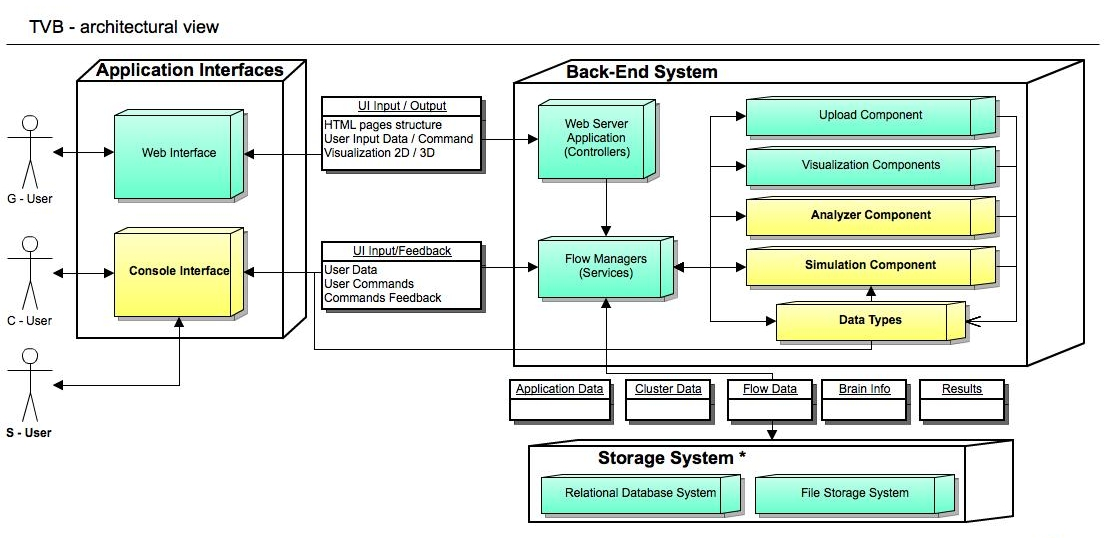
\includegraphics[width=0.90\textwidth]{images/architecture.jpg}
        \caption{TVB architecture: Yellow blocks are part of the Scientific
            Library of TVB, while the green blocks are part of TVB Framework.
            TVB provides two independent interfaces, depending on the
            interaction type wanted by the end-user (web or console).  TVB
            Storage layer is compulsory for the web interface, but it can be
            switched on/off for the console interface.  \note[lp]{It is said in
                the text that "console interface" is part of the "architecture"
            and not the "scientific library", this is the contrary on the
        figure}
        \note[lp]{What is a "S-User"? I missed the definition?}
         }
        \label{fig:architecture}
 \end{figure*}

 The goal of this article is firstly to decribre TVB framework from the
 development point of view and demonstrates how it interacts with other tools
 and how it can be extended (on the basis of extension already integrated in
 TVB).
